% Intended LaTeX compiler: pdflatex
\documentclass[10pt,a4paper,UTF8]{article}
\usepackage{zclorg}
\usepackage{tikztheorem}
\author{zcl.space}
\date{}
\title{弱大数定理}
\hypersetup{
 pdfauthor={zcl.space},
 pdftitle={弱大数定理},
 pdfkeywords={probability},
 pdfsubject={},
 pdfcreator={Emacs 25.0.50.1 (Org mode 9.0.6)},
 pdflang={English}}
\begin{document}

\maketitle
\tableofcontents
\titlepic{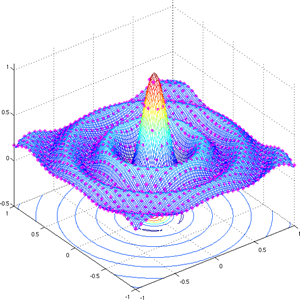
\includegraphics[scale=0.25]{../../img/sinc.PNG}}

\section{引子}
\label{sec:orge0f4e09}


在概率论中,极限定理是最重要的理论结果。在极限定理中最核心的结果是大数定理和中心极限定理。通常,大数定理是考虑随机变量序列的平均值收敛到某预期值。相比之下,中心极限定理证明大量随机变量之和的分布在某种条件下逼近于正态分布。

\section{马尔科夫不等式和切比雪夫不等式}
\label{sec:orgc3511dc}


首先引入马尔科夫不等式:
\begin{tikztheorem}
设\(X\)为取非负值的随机变量,则对于任何常数\(a > 0\),有:
\begin{equation}
\label{eq:1}
P\{ X \geq a \} \leq \frac{E[X]}{a}
\end{equation}
\end{tikztheorem}

\begin{tikzproof}
对于\(a > 0\),令:
\begin{equation}
\label{eq:2}
I =
\begin{cases}
1 & X \geq a\\
0 & \mathrm{others}
\end{cases}
\end{equation}
由于\(X\geq 0\),我们有:
\begin{equation}
\label{eq:3}
I \leq \frac{X}{a}
\end{equation}
对上述不等式两边求期望,得:
\begin{equation}
\label{eq:4}
\mathbb{E}[I] \leq \frac{1}{a}\mathbb{E}[X]
\end{equation}
因为\(\mathbb{E}[I] = P\{X\geq a\}\),所以命题得证。
\end{tikzproof}

\begin{tikztheorem}
设\(X\)是随机变量,均值\(\mu\)和方差\(\sigma^{2}\)都是有限值,则对任何\(k > 0\),有:
\begin{equation}
\label{eq:5}
P\{| X - \mu| \geq k\} \leq \frac{\sigma^{2}}{k^{2}}
\end{equation}
\end{tikztheorem}

\begin{tikzproof}
由于\((X-\mu)^{2}\)为非负随机变量,利用马尔科夫不等式\(a=k^{2}\),得:
\begin{equation}
\label{eq:6}
P\{ (X-\mu)^{2} \geq k^{2} \} \leq \frac{\mathbb{E}[ (X-\mu)^{2} ]}{k^{2}}
\end{equation}
由于\((X-\mu)^{2} \geq k^{2}\)与\(|X-\mu| \geq k\)是等价的,因此上式等价于:
\begin{equation}
\label{eq:7}
P\{ |X - \mu| \geq k \} \leq \frac{\mathbb{E}[(X-\mu)^{2}]}{k^{2}} = \frac{\sigma^{2}}{k^{2}}
\end{equation}
\end{tikzproof}

马尔科夫不等式和切比雪夫不等式的重要性在于,我们能够在只知道分布的期望或者只知道分布的期望和方差时,利用它们导出概率上界。当然,如果实际概率分布已知,我们可以直接计算准确的概率而不必推导概率上界。
\section{例子}
\label{sec:org60949d7}


\begin{tikzinstance}
假设已知某工厂在一周内生产的产品数量是一个均值为\(50\)的随机变量。
\begin{enumerate}
\item 本周内产品数量超过75件的概率是多少?
\item 如果我们进一步知道每周产量的方差为\(25\),那么本周产量在40到60之间的概率是多少?
\end{enumerate}
\end{tikzinstance}
\begin{tikzanswer}
记\(X\)为该工厂本周所生产的产品数量。
\begin{enumerate}
\item 由马尔科夫不等式,得:\[ P\{ X > 75\} \leq \frac{\mathbb{E}[X]}{75} = \frac{50}{75} = \frac{2}{3}\]
\item 由切比雪夫不等式,得:\[ P\{ |X-50| \geq 10 \} \leq \frac{\sigma^{2}}{10^{2}} =\frac{1}{4} \]所以\[P\{ |X -50| < 10 \}\geq 1- \frac{1}{4} = \frac{3}{4}\]
\end{enumerate}
\end{tikzanswer}

\begin{tikzinstance}
设随机变量\(X\)服从\((0,10)\)上的均匀分布,那么,因为\(\mathbb{E}[X] = 5, \mathrm{Var}[X]= 25/3\),所以利用切比雪夫不等式可得:
\begin{equation}
\label{eq:8}
P\{ |X-5| > 4 \} \leq \frac{25}{3\times 16} \approx 0.52
\end{equation}
而实际的概率值为:
\begin{equation}
\label{eq:9}
P\{ |X-5| > 4 \} = 0.20
\end{equation}
\end{tikzinstance}
从上面的例子可以看出,我们利用切比雪夫得到概率上界,但不能用它来估计概率值本身。因此,尽管切比雪夫不等式是正确的,但是它所导出的上界并不那么贴近实际概率值。切比雪夫的一个重要的应用体现在一些命题的证明过程中。

\begin{tikztheorem}
若\(\mathrm{Var}[X] = 0\),则:
\begin{equation}
\label{eq:10}
P\{X = \mathbb{E}[X]\} = 1
\end{equation}
换言之,一个随机变量的方差为零的充要条件是这个随机变量以概率1等于常数。
\end{tikztheorem}

\begin{tikzproof}
利用切比雪夫不等式,对任何\(n\geq 1\):
\begin{equation}
\label{eq:11}
P\{ |X - \mu| > \frac{1}{n} \} = 0
\end{equation}
令\(n\to \infty\),并应用概率的连续性性质,得:
\begin{equation}
\label{eq:12}
0 = \lim_{n\to\infty}P\{ |X-\mu| > \frac{1}{n} \} = P\{\lim_{n\to\infty}\{ |X-\mu| > \frac{1}{n} \}\} = P\{X\neq \mu\}
\end{equation}
得证。
\end{tikzproof}

\section{弱大数定理}
\label{sec:org496833a}


\begin{tikztheorem}
设\(X_{1},X_{2},\ldots\)为独立同分布的随机变量序列,其公共期望\(\mathbb{E}[X_{i}] = \mu\)有限,则对任何\(\epsilon > 0\):
\begin{equation}
\label{eq:13}
P\bigg\{ \bigg| \frac{X_{1}+ \ldots + X_{n}}{n} - \mu \bigg| \geq \epsilon \bigg\} \to 0 \qquad n\to \infty
\end{equation}
\end{tikztheorem}
\begin{tikzproof}
我们只在\(\mathrm{Var}[X_{i}] = \sigma^{2}\)有限的情形下证明此定理。此时,因为:
\begin{equation}
\label{eq:14}
\mathbb{E}\bigg[\frac{X_{1} +\ldots +X_{n}}{n}\bigg] = \mu, \qquad  \mathrm{Var}\bigg[ \frac{X_{1} +\ldots +X_{n}}{n} \bigg] = \frac{\sigma^{2}}{n}
\end{equation}
利用切比雪夫不等式,得:
\begin{equation}
\label{eq:15}
P\bigg\{ \bigg| \frac{X_{1}+ \ldots + X_{n}}{n} - \mu \bigg| \geq \epsilon \bigg\} \leq \frac{\sigma^{2}}{n\epsilon^{2}}
\end{equation}
得证。
\end{tikzproof}

弱大数定理最早是詹姆斯伯努利在\(X_{i}\)只取\(0\)或者\(1\)的特殊情况下证明的。
\end{document}
